\chapter{垂测电离图分割}
\label{cha3}
在上个章节中,主要介绍了电离层及电离层探测技术,并提出了本文算法流程图。本章主要介绍垂测电离图分割算法,包括将垂测电离层探测数据转换为电离图、电离图预处理、电离图E区F区分割算法。

%=============================================================================================================
\section{垂测数据转换为电离图}
\label{3_1}

本文实验中所采用的数据是由中国电波传播研究所自主研制的TYC-1型垂测仪采集的,采集的回波数据由电离层垂直反射信号和噪声信号构成,并以二进制的形式存储在文件中,利用数据的形成原理,我们可以将垂测数据转换为灰度电离图(320*640的二维矩阵)。
       
电离图的垂测数据文件格式:
\begin{enumerate} 
\item每次探测的数据保存在一个二进制文件中:文件名:yyyymmddHHMMp30s1.0h0.0V.O,文件名中的yyyy表示数据的采集年份、mm表示数据的采集月份、dd表示数据的采集日、HH表示数据的采集小时、MM表示数据的采集分钟,p后的数据表示频率步长$f_{step}$(KHz),s后的数据表示初始频率$f_{0}$(MHz),h后的数据表示起始高度$h_{0}$(km)。高度固定步长为2.5km。例如201110191400p35s1.0h0.0V.O表示2011年10月19日14时00分以初始频率为1MHz、步长为35KHz 采集的电离层二进制数据。

\item文件大小固定:302k=162×640+100000(字节)
         
\item162×640数据块的格式: 640个的频率点,$f_{0}$到$f_{0}+f_{step}*640$; 160×2个高度点为$h_{0}$到$h_{0}+2.5*160*2$。
\end{enumerate}   
 
将垂测数据转换为电离图的具体步骤如下:
 
\begin{enumerate}         
\item读取源数据,将数据转换为十进制并保存到一个大小为207462的数组中;
         
\item为了便于将数据转换为大小为$162\times1280$的图像,需要去掉尾部$207462-162\times1280=102$个字节的数据;
         
\item将长度为204800个元素组成的数组变为一个$160\times1280$的矩阵;
         
\item将矩阵的奇数列作为寻常波,将矩阵的偶数列作为非寻常波,得到两个大小为$160\times640$的寻常波与非寻常波矩阵;
         
\item将寻常波矩阵与非寻常波矩阵进行相加形成新矩阵,将矩阵的每一行进行复制,并插入被复制行的下一行,得到一个$320\times640$的矩阵,再将矩阵倒置就可得到垂测电离图原始图像。
\end{enumerate}  
        
为了观测电离层的变化,在我国大多数地区进行观测时都是每隔15分钟或半个小时对电离层进行一次探测,得到一组电离层探测数据。如图~\ref{图3_1}所示,原始的垂测电离图是由测高仪探测数据转换得到的,该图具有垂直测高仪探测到的全部电离图数据,由电离图可以看出各层电离层描迹保持了一定的几何形态、同时反映出了电离图各层的特征。

\begin{figure}[h]
\centering
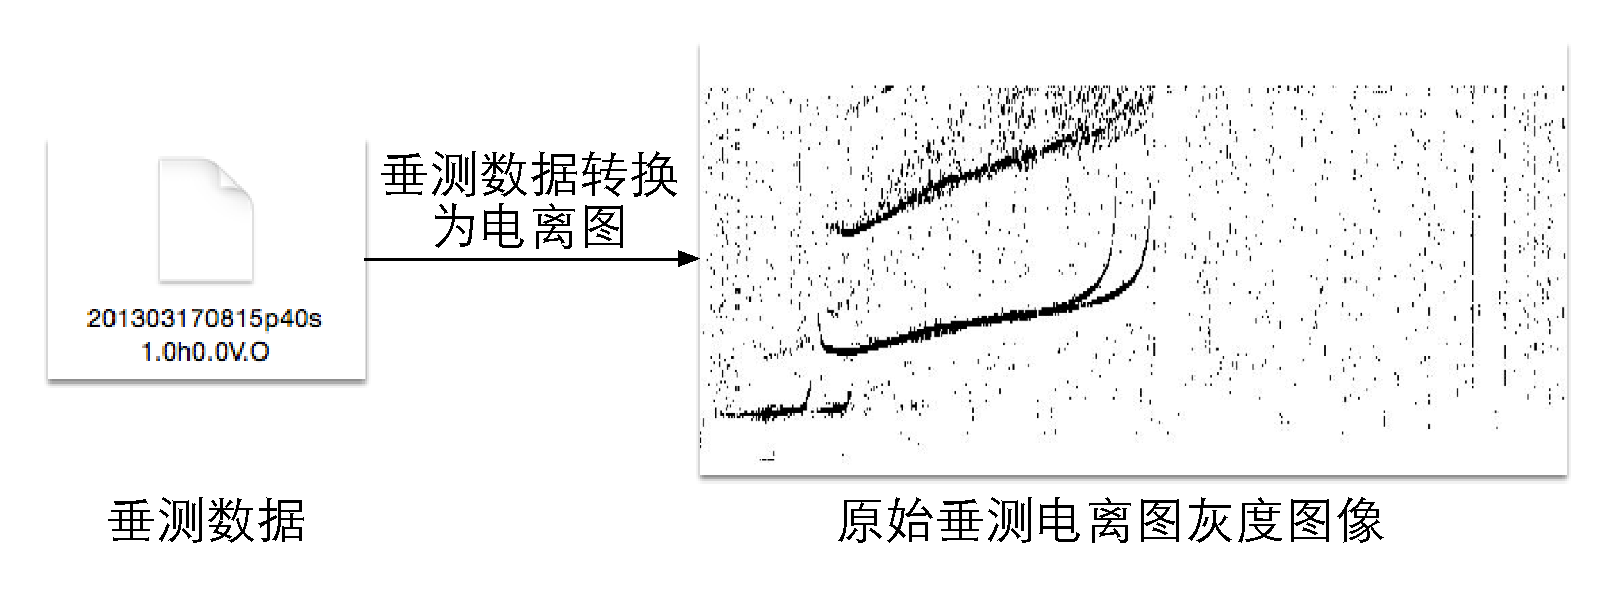
\includegraphics[height=4cm]{图3_1}
\caption{数据转换为电离图}
\label{图3_1}    
\end{figure}
 %=============================================================================================================
\section{电离图预处理}
\label{3_2}
电离图预处理操作对电离图E区F区的正确分割有重要作用。对电离图E区F区分割之前,首先对电离图进行预处理,去除电离图上的噪声。本文根据电离图所特有的噪声特点,从图像处理角度提出了电离图预处理方法。
         
因大量电离图存在垂线噪声,这些噪声会干扰F层临界频率的判读,所以先对电离图上的垂线噪声进行去除。本文中利用垂直投影法去除垂线噪声。 在上一步经垂测数据转换为灰度电离图,即电离图上每个信号点的取值范围为(0~255),为了便于计算垂直积分值,将灰度电离图转换为二值电离图。如果电离图上某像素点灰度值大于0,就将二值电离图上对应位置赋值为1;如果电离图上某像素点灰度值等于0,就将二值电离图上对应位置赋值为0。大小为m*n的二值电离图对应的灰度值函数用$I(x,y)$表示,那么第$y$列对应的垂直投影值为$VPV(y)=\sum_{x=1}^{m}I(x,y)$,计算电离图矩阵的每列的积分值,通过大量实验验证,我们选择70作为区分电离图上描迹和垂线噪声的阈值,当电离图上某列的积分值超过阈值就认为此列为垂线噪声,并在原电离图上将此列清零。如图~\ref{图3_2}为去除垂线噪声效果图。

\begin{figure}[h]
\centering
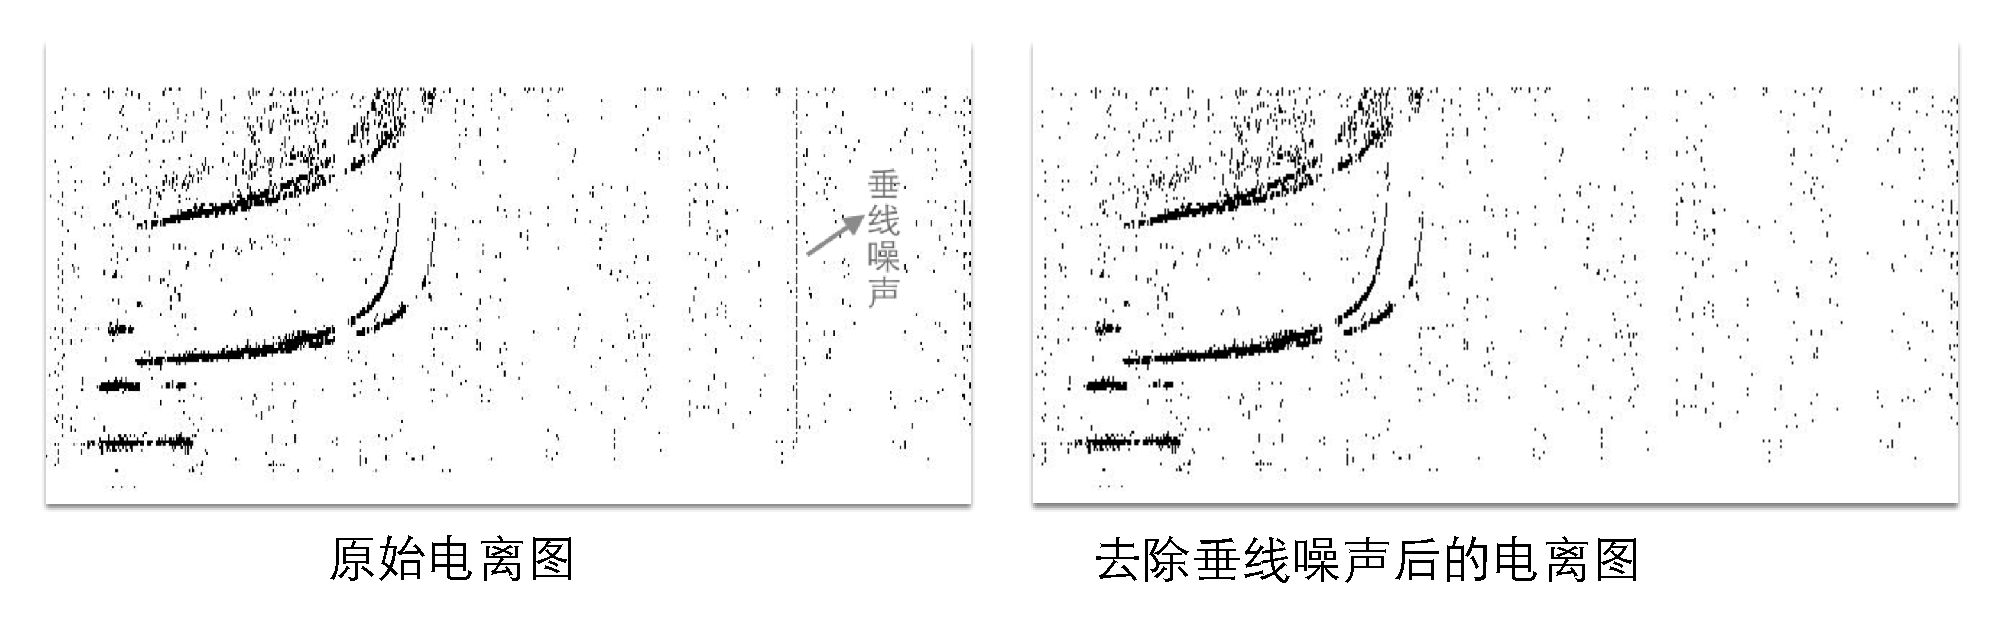
\includegraphics[height=4.5cm]{图3_2}
\caption{去除垂线噪声}
\label{图3_2}    
\end{figure}
  
电离图上每个像素点的灰度值大小代表探测数据信号的强弱,很难通过简单地根据像素值的大小,来区分描迹信号与电离图上的噪声。我们可以利用阈值滤波选取合适的灰度阈值,去除电离图上灰度值小于阈值的像素点,这样能够减少干扰噪声。
            
阈值分割对于区分图像上的目标和背景有重要作用。对电离图进行阈值分割可以很好的去除电离图上的噪声,同时保留描迹的重要信息。在阈值分割算法中,最关键的问题时如何为图像找到一个合适的阈值,如果阈值选择不适,可能将电离图上的描迹信息误认为噪声去掉或将噪声作为描迹信息保留。在计算分割阈值时,针对不同的图像特征,研究者会选择不同的图像特征来计算阈值,自动阈值分割方法划分为基于聚类、空间、目标等特征的多种方法\cite{sezgin2004survey}。
    
本文利用阈值分割对电离图上的描迹和噪声进行划分,将小于阈值的像素点作为噪声去掉,将大于阈值的像素点作为描迹。根据电离图像素灰度值分布特点,本文选择基于聚类的自动阈值方法进行阈值计算。基于聚类的自动阈值分割主要的方法有迭代法和最大类间方差法。迭代法计算出的阈值对物体边缘并很好的效果,同时如果图像的像素值发生波动,阈值也会发生相应变化,对分割结果产生影响。本文运用最大类间方差法对电离图进行阈值分割。
         
最大类间方差法\cite{otsu1975threshold},由日本的大津展之于1979年提出。根据图像的特征,将图像上的像素分为目标和背景两类,在两类之间存在类间方差,如果类间方差越大,说明目标和背景的差别越大,分割效果越好。运用概论统计知识找到使类间方差达到最大的灰度值作为分割阈值。
         
垂直探测电离图的信号幅度值范围为 $[0, L]$,那么某个像素值出现的概率为:
\begin{linenomath}
\begin{align}
P_{i}=\frac{n_{i}}{N},\quad i\in[0,L-1]
\label{式3_1}
\end{align}
\end{linenomath}
         
设背景像素属于A类,目标像素属于B类,坐标点$(x,y)$ 的像素灰度值为 $f(x,y)$。两类的概率和灰度均值分别为:
\begin{linenomath}
\begin{align}
P_{A}=\sum_{i=0}^{k}P_{i}  
\label{式3_2}
\end{align}
\end{linenomath}
\begin{linenomath}
\begin{align}
 \omega_{A}=\sum_{i=0}^{k}iP_{i}/P_{A}   
\label{式3_3}
\end{align}
\end{linenomath}  
\begin{linenomath}
\begin{align}
  P_{B}=\sum_{i=k+1}^{L-1}P_{i} 
\label{式3_4}
\end{align}
\end{linenomath}
\begin{linenomath}
\begin{align}
 \omega_{B}=\sum_{i=k+1}^{L-1}iP_{i}/P_{B} 
\label{式3_5}
\end{align}
\end{linenomath}

图像的灰度平均值为:
\begin{linenomath}
\begin{align}
\omega=\sum_{i=0}^{L-1}i*P_{i}
\label{式3_6}
\end{align}
\end{linenomath}

我们将最佳阈值定义为能得到最大类间方差的灰度值:
\begin{linenomath}
\begin{align}
t=argmax\{P_{A}(\omega_{A}-\omega)^2+P_{B}(\omega_{B}-\omega)^{2}\}
\label{式3_7}
\end{align}
\end{linenomath}


图像以$t$为阈值的分割结果表示为:
\begin{linenomath}
\begin{align}
f_t(x, y) = \left\{ \begin{array}{ll}
0 & f(x, y) < t\\
1 & f(x, y) \ge t
\end{array} \right.
\label{式3_8}
\end{align}
\end{linenomath}
           
将电离图中灰度值小于分割阈值的像素点划分为电离图描迹,其它像素点划分为噪声,通过该方法可以很好的去除电离图上的噪声。经过大量实验验证,运用最大类间方差法能够为垂测电离图找到合适的分割阈值,同时阈值一般非常稳定,利用阈值分割对图像进行预处理就可以很好的去除电离图上的离散噪声,减小干扰。因此本文选择运用大津法对电离图进行自动去噪。如图~\ref{图3_3}为电离图经过去除噪声和最大类间方差的阈值分割得到的电离图预处理结果。

\begin{figure}[h]
\centering
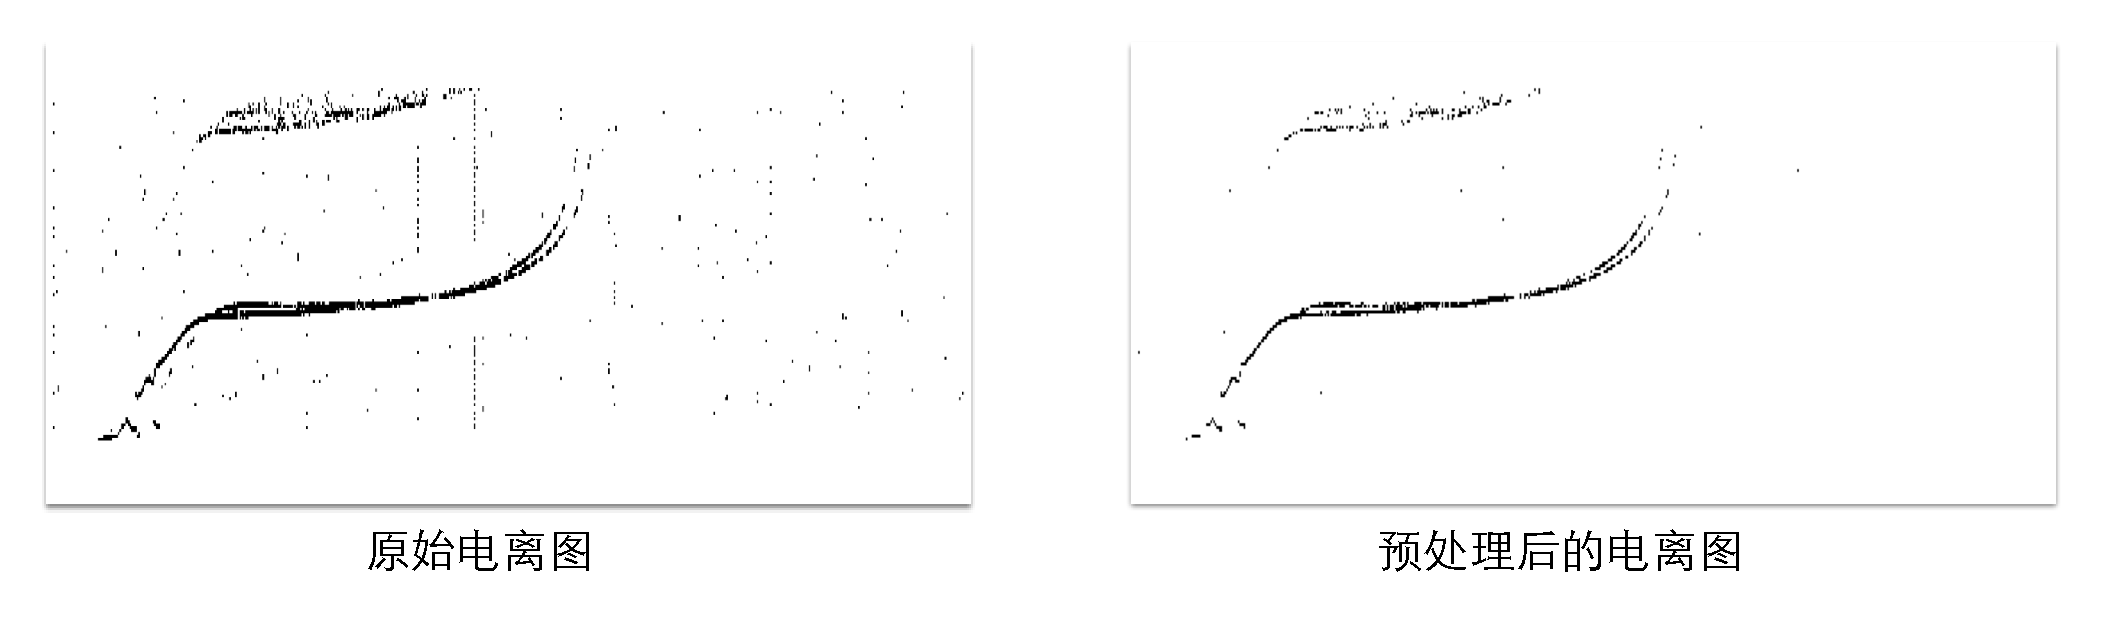
\includegraphics[height=4.3cm]{图3_3}
\caption{电离图预处理结果}
\label{图3_3}    
\end{figure}
 
因此,为了使电离图E区F区分割时找到合适的分割线,本文先对原始电离图进行预处理得到去除噪声的二值电离图。先去掉原始电离图上的垂线噪声,再利用最大类间方差法对电离图进行去噪。 

 %=============================================================================================================
\section{电离图E区F区分割}
\label{3_3}

正确的对电离图E区F区进行分割对电离图E区、F区描迹检测及简化后期算法的复杂度和更准确的度量电离图相关参数都有重要作用。本文将水平投影积分法、电离图的人工度量知识、电离图度量参数经验值共同运用到电离图E区F区分割算法中。
         
电离层F区内包括F层描迹及其反射和来自Es层描迹的多次反射,E区一般为E层、Es层、E2层描迹存在的区域。通过对大量电离图进行观察发现,在电离图E区和F区之间存在一定的无描迹区域,我们将这个区域称为E-F谷区,即垂直探测仪的探测盲区。所以本文的电离图E区F区分割算法利用水平投影积分法对电离图上的无描迹区域进行检测,并结合人工度量知识与经验确定电离图E区F区之间的最优分割线。
         
为了减少算法计算量并保证算法的准确性,需要设定一个包含各种情况下E区和F区分割线的参考区间。因F层的最低虚高可以为电离图E区、F区的分割线的选取提供标准,本文对中国不同地区和不同时段电离图的F层最低虚高的经验数据进行统计,确定了范围150km~350km(电离图矩阵的180行到260行)作为参考区间。
         
首先,利用水平投影积分法对参考区间内零区(即参考区间内没有信号点的连续行构成的区域)的个数进行统计,每张电离图的参考区间内可能存在多个零区,但是,每个零区形成的原因不尽相同,可能由于F层描迹的间断、未除掉的噪声、E区描迹的间断或E区与F区之间的间隙。
         
为了更好地判断零区是不是E区与F区的间隙,我们引入下面这些概念对零区的特征进行描述:
\begin{enumerate}          
\item零区宽度值($h_{width}^{'}$):如果零区位于电离图第$x1$行到第$x2$行,那么这个零区的宽度$h_{width}^{'}=h^{'}(x1)-h^{'}(x2)$;
         
\item非零区:有信号点的连续行构成的区域;
         
\item水平投影最大值(${HPV}_{max}$):对二值电离图$I(x,y)$进行水平投影积分,可以得到第$x$行对应的水平投影值,$HPV(x)=\sum_{y=1}^{n}I(x,y)$,那么$HPV_{max}=max(HPV)$;
         
\item水平投影最大值位置(${{h^{'}}_{HPV}}_{max}$):当$x=x^{*}$时,$HPV(x^{*})={HPV}_{max}$。$x^{*}$所对应虚高$h^{'}(x^{*})$,就是水平投影最大值位置。
\end{enumerate}    
      
然后,根据参考区间内零区个数,设计了不同的分割线查找方法。具体分割算法如图~\ref{图3_4}所示,

\begin{figure}[h]
\centering
\includegraphics[height=12cm]{图3_4}
\caption{电离图E区F区分割算法流程图}
\label{图3_4}    
\end{figure}
  
对于无零区电离图,取参考区间水平积分最小值对应的行(${x_{HPV}}_{min}$)作为电离图E区、F区的分割线。         
	 
对于一个零区电离图,该零区为电离图E区和F区之间的虚高间隙,取零区的中线作为电离图E区、F区的分割线。
	 
对于多个零区的电离图,我们主要通过对零区的特征值 ${{h^{'}}_{HPV}}_{max}$和$h_{width}^{'}$进行分析,排除描迹间断,选择最优零区作为E区和F区描迹间隙。具体算法如下:
\begin{enumerate}	 
\item查找电离图上非零区的(${{h^{'}}_{HPV}}_{max}$),即查找与参考区间内零区相邻且位于零区上面的非零区的${{h^{'}}_{HPV}}_{max}$。如图~\ref{图3_5}所示,位于参考区间内的零区有零区1和零区2,与零区相邻且位于零区上面的非零区为非零区1和非零区2。求非零区1和非零区2构成区域的${{h^{'}}_{HPV}}_{max}$,即在区间$[p1,p2]$内找到${{h^{'}}_{HPV}}_{max}$,通过计算,图~\ref{图3_5}的分割线位于341km处。

\begin{figure}[h]
\centering
\includegraphics[height=8cm]{图3_5}
\caption{E区F区分割图例}
\label{图3_5}    
\end{figure}

\item根据非零区的${{h^{'}}_{HPV}}_{max}$进一步定位分割线。$HPV_{max}$可能位于F层、Es层l型或f型描迹的二次反射、Es层n型描迹,根据这些描迹虚高的经验值,设定180km作为阈值对分割线进一步定位:a) 如果${{h^{'}}_{HPV}}_{max}>180km$,$HPV_{max}$位于F层、Es层l型或f型描迹的二次反射上,因此分割线位于${{h^{'}}_{HPV}}_{max}$下面的零区中;b) 如果${{h^{'}}_{HPV}}_{max} \leq180km$,$HPV_{max}$位于Es层n型描迹上,因此分割线位于${{h^{'}}_{HPV}}_{max}$上面的零区中。
		
\item在上一步定位的零区中,进行最优零区(E区F区描迹间隙)查找。我们利用零区的$h_{width}^{'}$特征来判断零区是不是描迹的间断,根据大量电离图数据的统计结果,设定区分E区和F区之间的描迹间隙与描迹间断之间的阈值为20km。如果在上一步定位的零区中存在$h_{width}^{'}>20km$的零区,选择距离${{h^{'}}_{HPV}}_{max}$最近且$h_{width}^{'}>20km$的零区作为最优零区;否则,选取上一步定位的零区中最宽的零区作为最优零区。	

\item将最优零区的中线作为E区F区的分割线。
	
\end{enumerate}  

如图~\ref{图3_5}所示,$HPV_{max}$(投影最大值)位于F层,E区F区分割线应位于${{h^{'}}_{HPV}}_{max}$下面的零区中。根据$h_{width}^{'}$可知,零区1为F层描迹的间断,故认为零区2为E区和F区之间的描迹间隙并将其中线作为E区F区的分割线。此方法可以避免由于F层描迹间断、噪声以及E区描迹间断等造成的分割错误,能够更加有效的进行E区F区分割。


%=============================================================================================================
\section{本章小结}
\label{3_4}

本章主要介绍了电离图E区F区分割算法,其中包括垂测数据转换为电离图、电离图预处理、电离图E区F区分割。运用本文算法对不同地区和不同时间段的49678张电离图进行实验,E区F区分割错误的电离图有1286张,正确率为97.41\%。


